\section{Introduction}

For the second experimental activity in the Circuit Theory and Electronics Fundamentals course, we were given a RC circuit to analyse.
This circuit is constituted by a sinusoidal voltage source $v_s$, dependent voltage $V_d$ and current $I_b$ sources, a capacitor $C$ and 7 resistors (fig. \ref{intro}).

The theoretical analysis (Section \ref{sec:analysis}) adresses, sequencially, the nodal analysis, then the calculus of $R_{eq}$. With these results, the natural response of the circuit, the forced response are computed, and then superimposed.

The simulation analysis (Section \ref{simuanal}) was made to validate the results obtained in section \ref{sec:analysis}, operating point, transient and then frequency analysis were made in Ngspice.
The conclusions of this study are outlined in the final section (\ref{resan}).

The voltage source varies in time as it follows:



\begin{equation}
v_s(t) = V_s u(-t) + sin(2\pi ft)u(t)
\end{equation}
where
\begin{equation}
u(t)=\begin{cases} 0, \quad t<0 \\ 1, \quad t \geq 0  \end{cases}
\end{equation}


To obtain the initial data, we ran a python script provided by our teacher, which generated the following data:\\

\begin{table}[h]
\centering
\begin{tabularx}{0.6\textwidth} {
  | >{\raggedright\arraybackslash}X
  | >{\raggedleft\arraybackslash}X | }
 \hline
R1 & 1.048998e+03 kOhm\\ \hline
R2 & 2.055568e+03 kOhm\\ \hline
R3 & 3.060188e+03 kOhm\\ \hline
R4 & 4.168980e+03 kOhm\\ \hline
R5 & 3.073950e+03 kOhm\\ \hline
R6 & 2.042810e+03 kOhm\\ \hline
R7 & 1.037563e+03 kOhm\\ \hline
Vs & 5.114229e+00 V\\ \hline
C & 1.011550e-06 uF\\ \hline
Kb & 7.338555e-03 mS\\ \hline
Kd & 8.258180e+03 kOhm\\ \hline

\end{tabularx}
\caption{Initial Data generated by the python script. The variables are expressed in V, mA, mS, kOhm, uF.}
\end{table}

\begin{figure}[ht] \centering
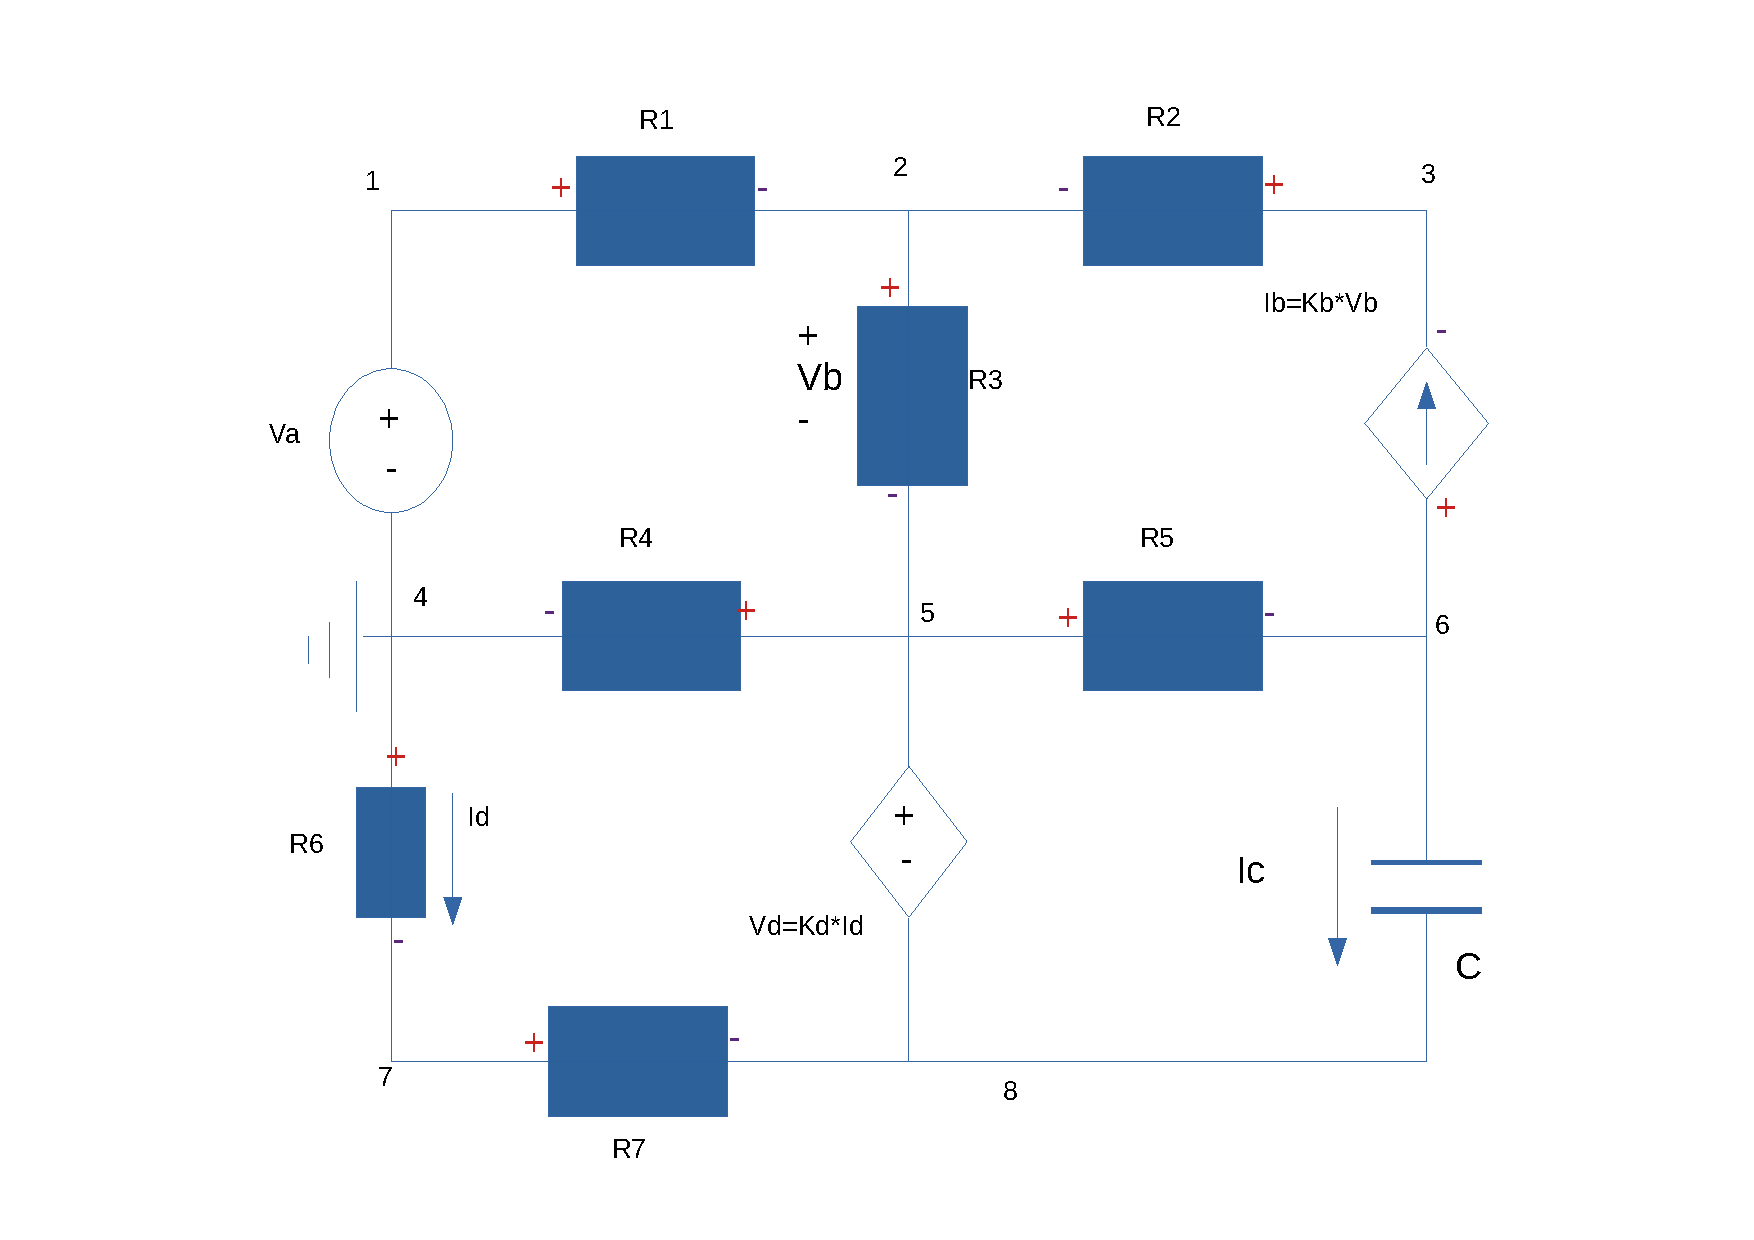
\includegraphics[width=0.7\linewidth]{Circuito1.pdf}
\caption{First Circuit}
\label{fig:snat}
\end{figure}

\begin{figure}[ht] \centering
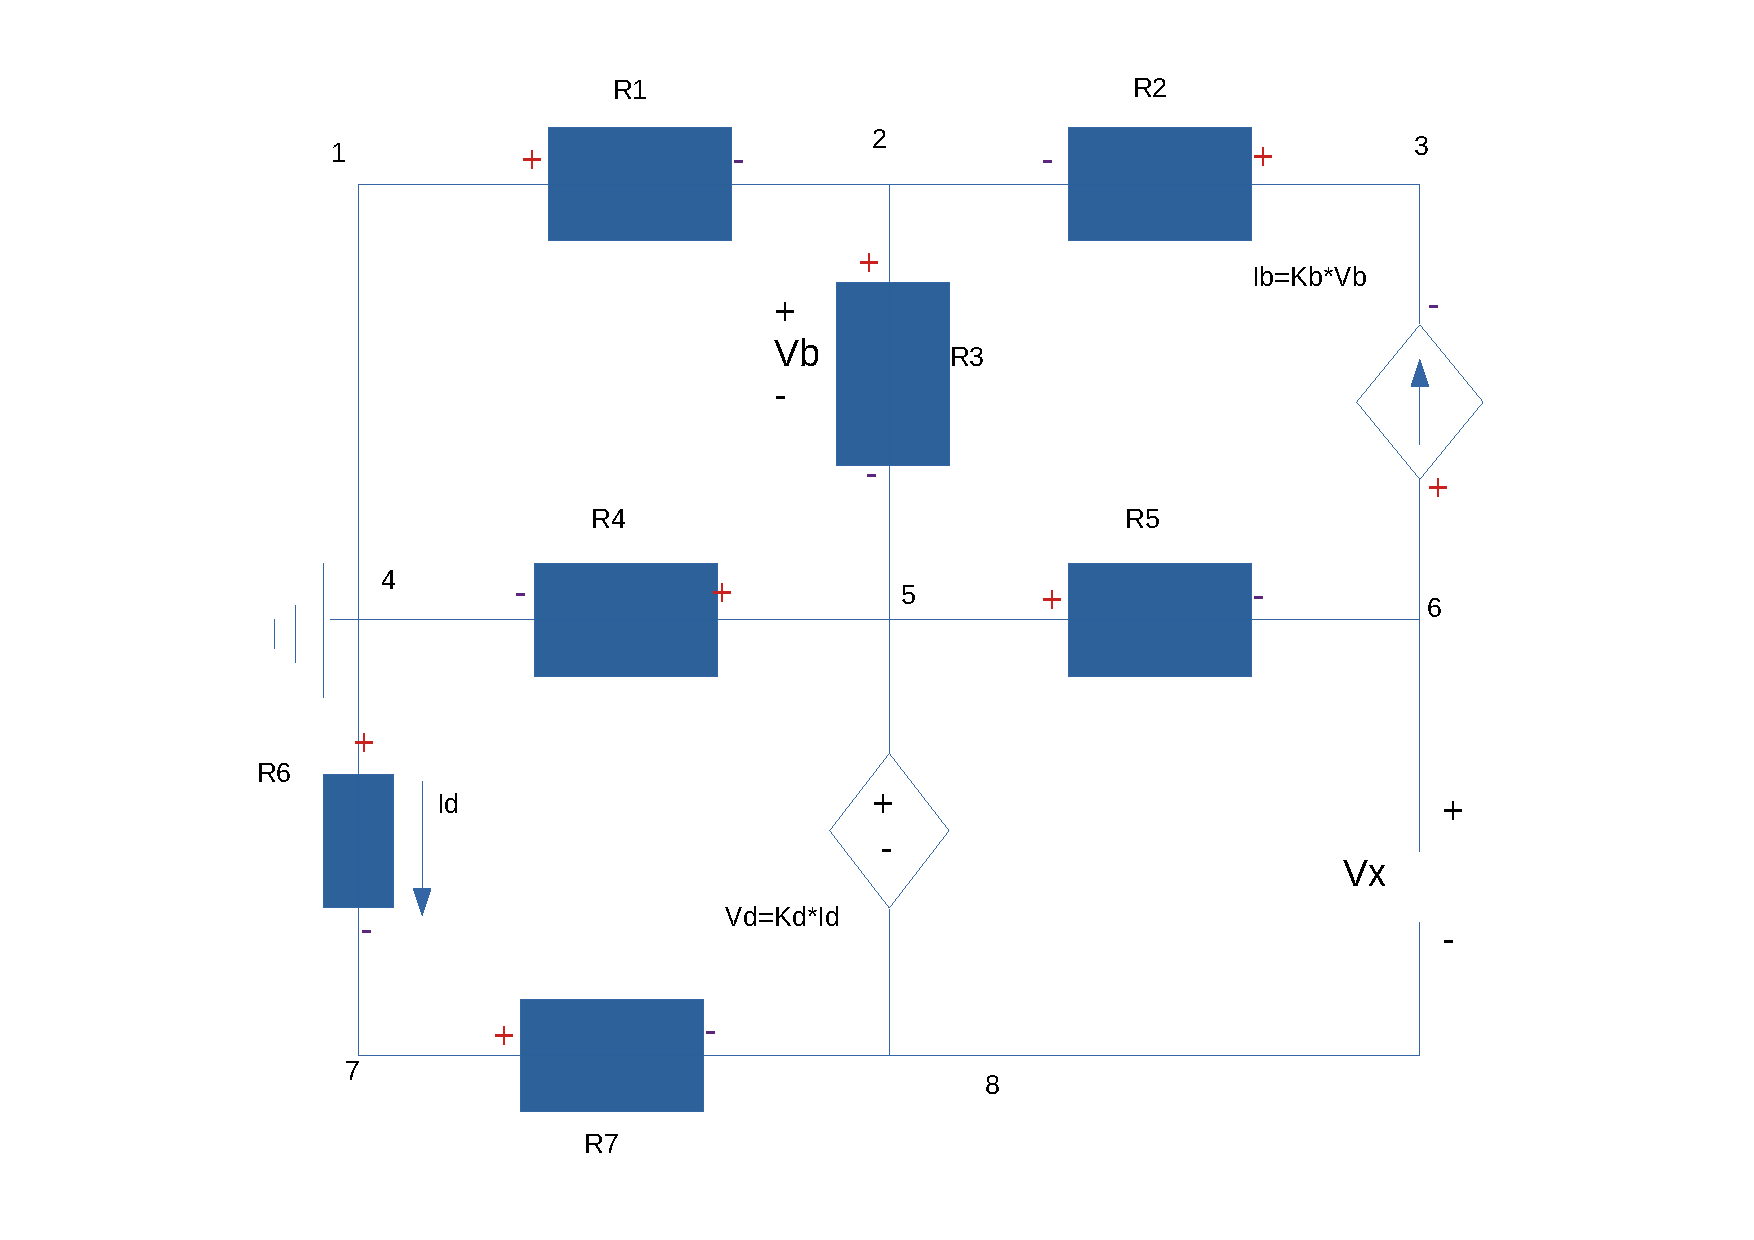
\includegraphics[width=0.7\linewidth]{Circuito2.pdf}
\caption{Second Circuit}
\label{fig:snat}
\end{figure}

\clearpage
